\section{The Observability Maturity Model (OMM)}
\label{sec:omm}

As a direct outcome of the Rapid Review conducted to address Specific Objective \textbf{SO4}, this research formalizes and proposes the \textit{Observability Maturity Model} (OMM). Maturity models are widely recognized in software engineering and IT service management as effective instruments for assessing organizational capabilities, diagnosing operational gaps, and guiding staged process improvements \cite{proenca_2016}. However, within the Information Systems (IS) literature, maturity models must not be treated as simple, ad-hoc checklists; rather, they represent complex, multi-dimensional **design artifacts** that require rigorous conceptual design, clear boundary definitions, and empirical validation \cite{mettler_2011}.

To establish a solid scientific foundation for the OMM, this research adopts a hybrid methodological framework combining the procedure design guidelines of \citeonline{becker_2009}, the design science research perspective of \citeonline{mettler_2011}, and the developmental lifecycle model of \citeonline{debruin_2005}.

\subsection{Methodological Design and Requirements Alignment}
According to \citeonline{becker_2009}, the development of a scientifically rigorous maturity model must satisfy eight fundamental design requirements to ensure its reliability and academic validity. Table \ref{tab:omm-becker-alignment} outlines how the OMM aligns with and satisfies each of these requirements.

\begin{table}[ht]
\centering
\footnotesize
\caption{OMM Alignment with Becker et al. (2009) Design Requirements}
\label{tab:omm-becker-alignment}
\begin{tabularx}{\textwidth}{|l|X|}
\hline
\textbf{Design Requirement} & \textbf{OMM Instantiation in this Thesis} \\ \hline
1. Comparison with existing models & Our literature synthesis (Chapter 3) mapped existing siloed APM/monitoring maturity models, highlighting the lack of cloud-native and correlation-focused frameworks. \\ \hline
2. Iterative research strategy & The OMM was refined cyclically across the design and prototyping phases of the PANOPTES architecture. \\ \hline
3. Evaluation & The model's target state (Level 4) is evaluated through a controlled experiment using Chaos Engineering (Chapter 7). \\ \hline
4. Multi-method presentation & Developed via a systematic literature synthesis (Rapid Review) and evaluated via quantitative systems engineering experiments. \\ \hline
5. Detailed documentation & All stages of the design, metric definitions, and evaluation scripts are fully documented and public. \\ \hline
6. Target audience definition & The model explicitly targets Site Reliability Engineers (SREs), system architects, and operations managers. \\ \hline
7. Problem definition & Addresses the complexity and fragmentation of telemetry data ($Metrics, Logs, Traces, Events$) in ephemeral Kubernetes environments. \\ \hline
8. Design results & Delivers a prescriptive framework capable of guiding organizations from siloed monitoring to unified, correlated observability. \\ \hline
\end{tabularx}
\par\medskip
\ABNTEXfontereduzida\selectfont\textbf{Source:} Developed by author (2026)
\end{table}

Furthermore, \citeonline{mettler_2011} argues that maturity models must be conceptualized as decision-support artifacts that assist managers in organizational design. By leveraging the three purposes of use defined by \citeonline{debruin_2005}, the OMM is structured to evolve through three distinct utilitarian stages:
\begin{itemize}
    \item \textbf{Descriptive Utility:} Act as a diagnostic tool to assess the current "as-is" state of a Kubernetes cluster's telemetry pipelines, isolating unindexed logs and missing distributed traces.
    \item \textbf{Prescriptive Utility:} Provides a clear, actionable evolutionary roadmap. The PANOPTES reference architecture acts as the prescriptive engineering vehicle designed to elevate a cluster from lower levels to Level 4 (Optimized).
    \item \textbf{Comparative Utility:} Enables future benchmarking by allowing organizations to compare their diagnostic efficiency ($MTTDiag$) against the resource overhead footprint ($CPU/Memory$), establishing comparative trade-offs.
\end{itemize}

\subsection{The Development Phases of OMM and the Validation Gap}
To construct and validate the model, this work follows the six-stage developmental framework proposed by \citeonline{debruin_2005}. Figure \ref{fig:model-dev-phases} illustrates this lifecycle, which we operationalize as follows:

\begin{figure}[ht]
    \centering
    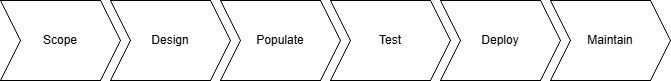
\includegraphics[width=1.0\linewidth]{images/observability/model-development-phases.png}
    \caption{Maturity Model Development Lifecycle (De Bruin et al., 2005)}
    \label{fig:model-dev-phases}
    \par\medskip\ABNTEXfontereduzida\selectfont\textbf{Source:} \citeonline{debruin_2005} \par\medskip
\end{figure}

\begin{itemize}
    \item \textbf{Scope:} Defined as a domain-specific model focusing exclusively on cloud-native containerized applications orchestrated by Kubernetes, addressing the architectural gaps in correlating multi-signal telemetry data.
    
    \item \textbf{Design:} Employs a multi-dimensional, stage-based linear architecture. It defines the telemetry space mathematically as the set $O = \{M, L, T, E\}$—representing Metrics, Logs, Traces, and Events, respectively—and evaluates capability across three layers: ingestion, storage correlation, and diagnostic retrieval.
    
    \item \textbf{Populate:} Achieved through a hybrid approach combining top-down stage definitions with a bottom-up population of capabilities, synthesized from the 237 primary studies identified in the Rapid Review.
    
    \item \textbf{Test (Mitigating the Validation Gap):} In a seminal systematic mapping study, \citeonline{wendler_2012} analyzed 237 maturity model publications and identified a critical research gap: **the Validation Gap**. The vast majority of academe-designed maturity models are published with speculative, qualitative evaluations (e.g., self-assertions or unvalidated case studies), lacking empirical, repeatable, and quantitative validation of their target states. 
    
    Our research directly mitigates this Validation Gap. We subject the model's target state (\textbf{Level 4 - Optimized}) to an exhaustive, automated, and controlled system-level experiment (Chapter 6 \& 7). By executing $N=30$ runs under randomized chaos (using Chaos Mesh), we provide empirical, statistically sound proof (using Mann-Whitney U testing) that transitioning to Level 4 capabilities reduces the Mean Time to Diagnose ($MTTDiag$) without violating resource bounds.
    
    \item \textbf{Deploy:} Instantiated and shared with the research and DevOps communities as reproducible open-source Infrastructure as Code artifacts (Multipass, Ansible, and Helm charts), enabling immediate replication and adoption.
    
    \item \textbf{Maintain:} Designed with an open capability architecture that anticipates technological evolution. It establishes Level 4 as the necessary data substrate required to support Level 5 (Predictive) AIOps models, which cannot function without correlated, high-fidelity traces and logs.
\end{itemize}

\subsection{OMM Evolutionary Levels}
As a result of the \textit{Scope}, \textit{Design}, and \textit{Populate} phases, we formalize the OMM across five cumulative levels of maturity, mapping the operational state of the telemetry set $O = \{M, L, T, E\}$:

\begin{enumerate}
    \item \textbf{Level 1 - Non-Existent:} The system is a complete black box. Telemetry data $O = \emptyset$. No logs, traces, or metrics are systematically collected. Troubleshooting is purely reactive, relying on user complaints and manual container restarts.
    
    \item \textbf{Level 2 - Initial/Ad-Hoc:} Characterized by siloed and fragmented telemetry ($O = \{M_{\text{local}}, L_{\text{local}}\}$). Metrics and container logs are scraped on-demand or stored locally within ephemeral nodes. Distributed traces are completely absent ($T = \emptyset$). Isolating cascading failures requires unindexed manual log searching, causing high cognitive load and long, non-deterministic diagnostic cycles.
    
    \item \textbf{Level 3 - Managed (Centralized):} Centralized collection is established ($O = \{M_{\text{central}}, L_{\text{central}}, T_{\text{siloed}}\}$). A telemetry collector aggregates data into distinct storage backends (e.g., separate databases for logs, metrics, and traces). While data is centralized, the signals remain un-correlated. Site Reliability Engineers (SREs) must manually pivot between different visualization tools or copy-paste trace IDs to correlate anomalies.
    
    \item \textbf{Level 4 - Optimized (Correlated - The PANOPTES Target):} Fully correlated, multi-modal telemetry is operationalized ($O = \{M \bowtie L \bowtie T \bowtie E\}$). The telemetry pipeline enforces strict semantic binding, linking metrics to traces using exemplars, and traces to logs using contextual span metadata. SREs navigate a single pane of glass, accelerating fault isolation. The empirical validity of this stage's diagnostic superiority is the core contribution of this thesis.
    
    \item \textbf{Level 5 - Predictive (AIOps):} Telemetry streams feed autonomous, intelligent closed-loop control agents ($O = f(M, L, T, E) \rightarrow \text{Control Action}$). Machine learning, variational autoencoders, and causal inference models ingest the high-fidelity correlated datasets provided by Level 4 to predict anomalies, execute auto-remediation, and dynamically scale resources before failure cascades impact end-users.
\end{enumerate}

By formalizing these evolutionary stages, the OMM provides a clear, scientifically grounded roadmap that helps researchers and practitioners navigate the complex landscape of cloud-native systems, positioning the PANOPTES architecture as the structural bridge to high-maturity operations.